\documentclass[a4paper]{jpconf}
\usepackage{graphicx}
\usepackage{comment}
\usepackage{subfig}
\usepackage{amssymb,amsmath}
\bibliographystyle{iopart-num}
%\usepackage{citesort}

%particles
\newcommand{\jpsi}{\rm J/$\psi$}
\newcommand{\psip}{$\psi^\prime$}
\newcommand{\jpsiDY}{\rm J/$\psi$\,/\,DY}
\newcommand{\chic}{$\chi_{\rm c}$}
\newcommand{\pip}{$\pi^{+}$}
\newcommand{\pim}{$\pi^{-}$}
\newcommand{\pizero}{$\pi^{0}$}
\newcommand{\kap}{K$^{+}$}
\newcommand{\kam}{K$^{-}$}
\newcommand{\pbar}{$\rm\overline{p}$}
\newcommand{\ccbar}{\ensuremath{\mathrm{c\overline{c}}}}
\newcommand{\bbbar}{\ensuremath{\mathrm{b\overline{b}}}}
\newcommand{\Dzero}{\ensuremath{\mathrm{D^{0}}}}
\newcommand{\Dzerobar}{\ensuremath{\mathrm{\overline{D}^{0}}}}
\newcommand{\Dpm}{\ensuremath{\mathrm{D^{\pm}}}}
\newcommand{\Ds}{\ensuremath{\mathrm{D_{s}^{\pm}}}}
\newcommand{\Dstar}{\ensuremath{\mathrm{D^{*\pm}}}}

%collision systems
\newcommand{\pp}{pp}
\newcommand{\pPb}{p--Pb}
\newcommand{\PbPb}{Pb--Pb}

%detectors
\newcommand{\ezdc}{$E_{\rm ZDC}$}

%units
\newcommand{\GeVc}{GeV/$c$}
\newcommand{\GeVcsq}{GeV/$c^2$}

%others
\newcommand{\degree}{$^{\rm o}$}
\newcommand{\s}{\ensuremath{\sqrt{s}}}
\newcommand{\snn}{\ensuremath{\sqrt{s_{\rm NN}}}}
\newcommand{\y}{\ensuremath{y}}
\newcommand{\pt}{\ensuremath{p_{\rm T}}}
\newcommand{\dedx}{d$E$/d$x$}
\newcommand{\dndy}{d$N$/d$y$}
\newcommand{\dndydpt}{${\rm d}^2N/({\rm d}y {\rm d}p_{\rm t})$}
\newcommand{\zpar}{\ensuremath{z_{||}}}
\newcommand{\zpargen}{\ensuremath{z_{||}^{\mathrm{part}}}}
\newcommand{\zpardet}{\ensuremath{z_{||}^{\mathrm{det}}}}
\newcommand{\ptchjet}{\ensuremath{p_{\mathrm{T,ch\, jet}}}}
\newcommand{\ptjet}{\ensuremath{p_{\mathrm{T,jet}}}}
\newcommand{\ptchjetgen}{\ensuremath{p_{\mathrm{T,ch\,jet}}^{\mathrm{part}}}}
\newcommand{\ptchjetdet}{\ensuremath{p_{\mathrm{T,ch\,jet}}^{\mathrm{det}}}}
\newcommand{\ptd}{\ensuremath{p_{\mathrm{T,D}}}}
\newcommand{\ptdgen}{\ensuremath{p_{\mathrm{T,D}}^{\mathrm{part}}}}
\newcommand{\ptddet}{\ensuremath{p_{\mathrm{T,D}}^{\mathrm{det}}}}
\newcommand{\antikt}{anti-\ensuremath{k_{\mathrm{T}}}}
\newcommand{\Antikt}{Anti-\ensuremath{k_{\mathrm{T}}}}
\newcommand{\kt}{\ensuremath{k_{\mathrm{T}}}}
\newcommand{\pthard}{\ensuremath{p_{\mathrm{T,hard}}}}

\begin{document}
\title{Measurement of jet \pT{} spectra in Pb--Pb collisions at $\snn=2.76~\mathrm{TeV}$ with the ALICE detector at the LHC}

\author{Salvatore Aiola$^{1,2}$}

\address{$^1$ University of Catania and INFN Sezione di Catania,  95123 Catania, Italy}
\address{$^2$ Lawrence Berkeley National Laboratory, Berkeley, CA 94720}

\ead{Salvatore.Aiola@cern.ch}

\begin{abstract}
Reconstruction of jets in high-energy heavy-ion collisions is challenging due to the large and fluctuating
background coming from the underlying event. We report results on full jet reconstruction, 
obtained from data collected in 2011 by the ALICE detector at LHC for \mbox{Pb--Pb} collisions 
at $\snn=2.76$~TeV. The analysis makes use of the tracking system and the electromagnetic calorimeter.
Signal jets, which come from hard scattered partons, are reconstructed using the \antikt{} jet finder algorithm. 
The average background is subtracted on a jet-by-jet basis to 
reduce the contribution to the jet reconstructed energy coming from the underlying event. The jet spectrum 
is corrected to account for fluctuations in the background momentum density and detector effects through 
unfolding.
\end{abstract}

\section{Introduction}
QCD jets are produced in high-energy particle collisions as a result of the fragmentation of a high momentum scattered parton.
Experimentally they are reconstructed using a well-defined algorithm, which acts as a working definition of a jet, to be used
consistently also in phenomenological models.
In heavy-ion collisions, hard 
scattered partons are produced in the early stages of the collision, so that they propagate through 
(and potentially are affected by) the hot and dense nuclear medium. The interactions suffered by 
the parton can result in energy loss, widening and/or complete absorption of jets. These phenomena go under the name
of ``jet quenching''.
RHIC and LHC experiments have already collected convincing evidence of jet quenching in a 
number of measurements, such as the suppression
of high-\pT{} particles relative to a pp baseline~\cite{hadrons-star-03,hadrons-phenix-04,hadrons-alice-10,hadrons-cms-12}, 
hadron-hadron correlations~\cite{dijet-star-06,dijet-alice-12}
and jet-jet correlations at high-\pT{}~\cite{dijet-atlas-10,jet-cms-11}. However, performing
a full jet reconstruction in the low and intermediate \pT{} region is particularly challenging due to the overwhelming soft particle background 
coming from the underlying event (UE). ALICE has recently reported
on a first detailed study of the background for jet reconstruction in the heavy-ion environment~\cite{bkg-alice-12}.

In these proceedings the analysis techniques utilized to fully reconstruct jets in Pb--Pb collisions with the 
ALICE experiment are presented. The results shown here come from data collected by ALICE in fall 2011 at $\snn=2.76$~TeV.

\section{Inputs to the jet finder}
The ALICE tracking system benefits of
the Inner Tracking System, a six-layer silicon detector which provides a precise measurement 
of the primary vertex together with the first points 
of the tracks, and of a large Time Projection Chamber~\cite{alice-08}. 
\begin{comment}
The tracking system allows reconstruction 
of charged tracks ranging from very low momentum 
($\pT\approx 0.15$~GeV/$c$) to high momentum ($\pT\approx 100$~GeV/$c$), 
with good momentum resolution and tracking efficiency.
\end{comment}
Tracks are reconstructed at mid-rapidity ($|\eta|<0.9$) and in full azimuth.
The ALICE electromagnetic calorimeter~\cite{ppr-emcal} is a Pb-scintillator sampling calorimeter, which covers mid-rapidity
($|\eta|<0.7$) and partial azimuth ($\Delta\phi=100^{\circ}$). The EMCal measures photons, e.g. from $\pi^0$ decays, which are
included in the jet finder input.
The shift of the jet energy scale due to 
unreconstructed particles, such as $K^0_L$ and neutrons, has been studied in pp simulations and 
accounted for in the final result.
\begin{comment}
Energy deposit in the calorimeter is pre-clusterized
prior to be utilized in the analysis. The clusterizer essentially put towers together such that each cluster contains only one local maximum. 
Charged particles also deposit some energy in the calorimeter. To avoid double counting
of this component of the energy, a correction procedure is applied on a cluster-by-cluster basis, after matching with charged tracks. Clusters
with a minimum transverse energy deposit of $0.3$~GeV (after charged energy subtraction) are accepted.
While electrons and positrons
showers are well-contained in the calorimeter, except at very high energies ($E_{\rm T}>100$~GeV), 
the response to charged hadrons is quite broad
and includes MIP deposition together with partially contained hadronic showers. 
\end{comment}
A full description of the ALICE experiment is available in Ref.~\cite{alice-08}.

\section{Jet finding and average background}
\begin{figure}[t]
\centering
\subfloat[][$R=0.2$.]
{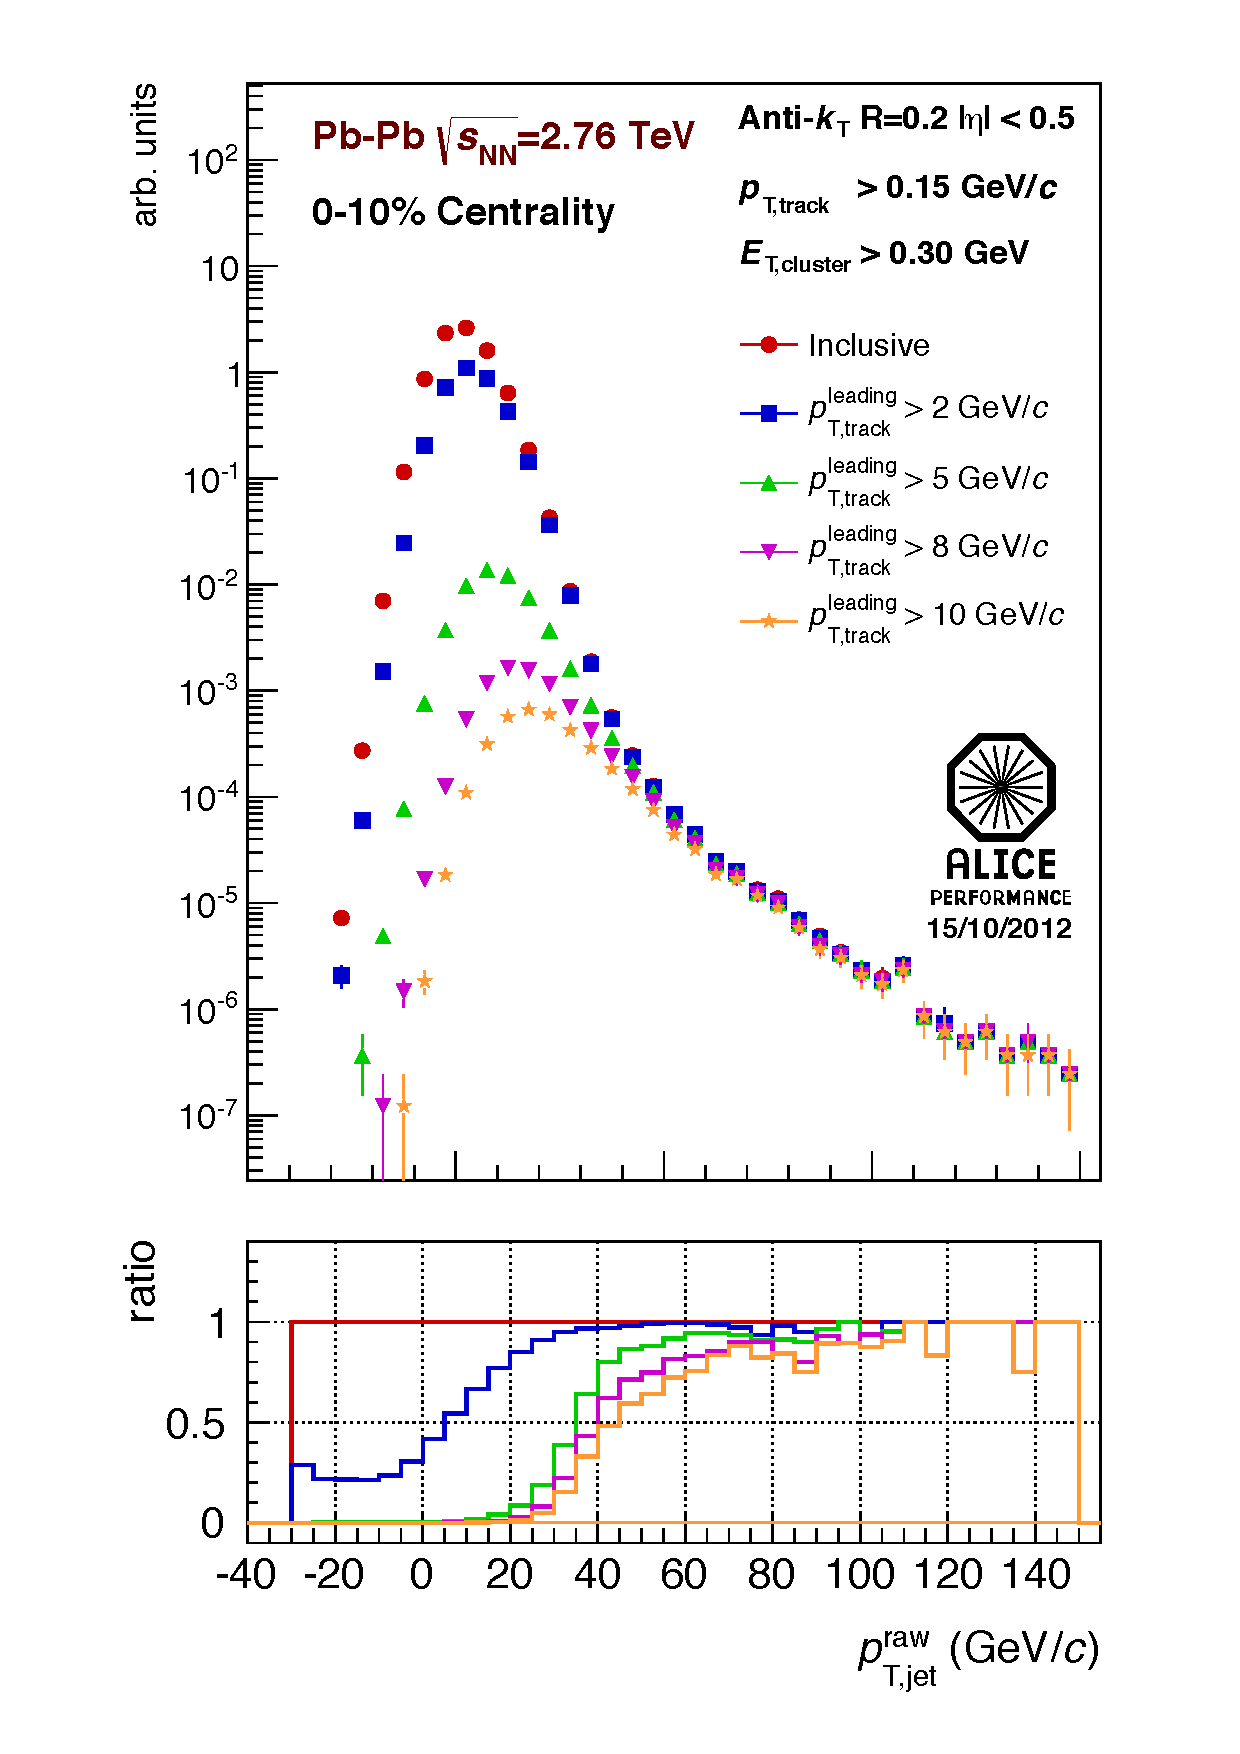
\includegraphics[width=.4\columnwidth]{RawJetSpectraPtR02}} \quad
\subfloat[][$R=0.3$.]
{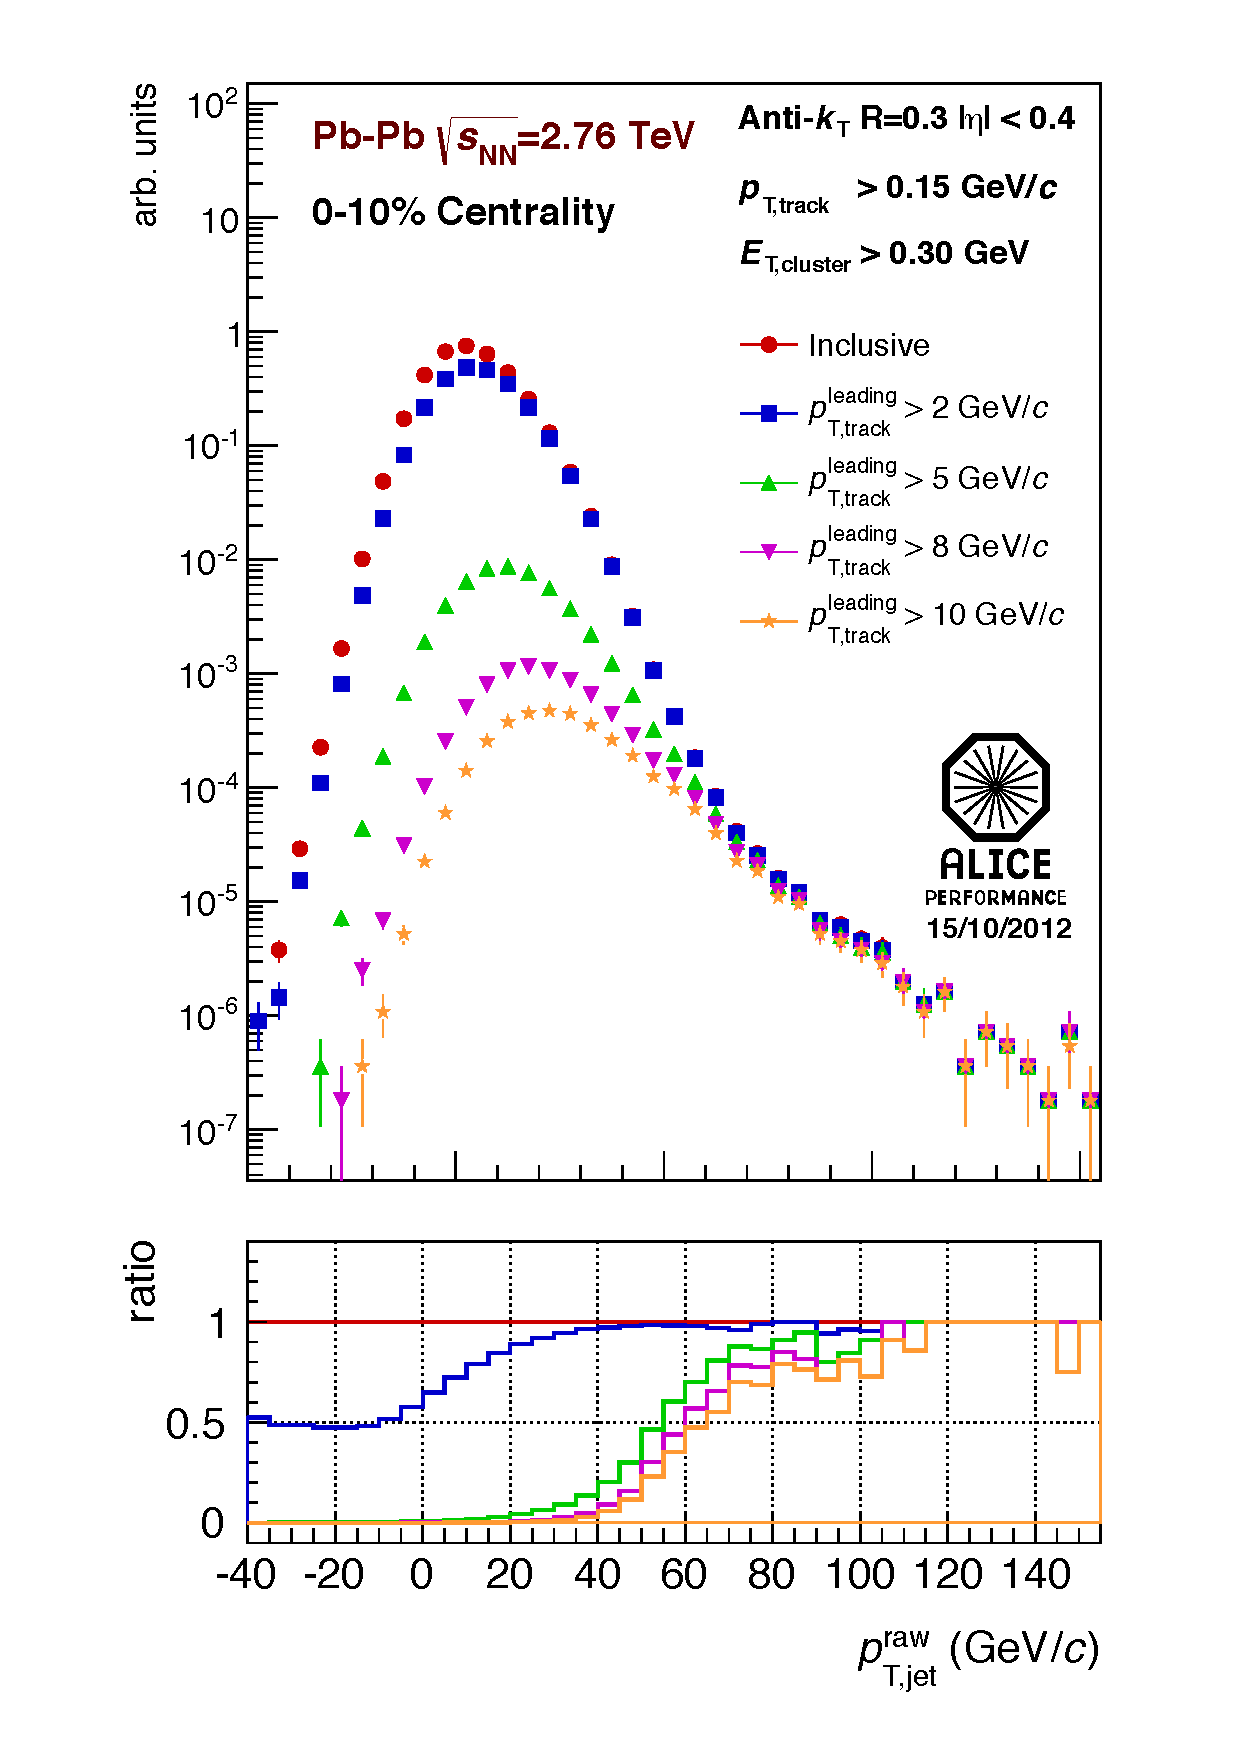
\includegraphics[width=.4\columnwidth]{RawJetSpectraPtR03}} 
\caption{Raw jet \pT{} spectra in \mbox{Pb--Pb} collisions at $\snn=2.76$~TeV in the 0-10\% centrality range at mid-rapidity:
inclusive is shown in full circles and with 
increasing minimum leading hadron \pT{} requirement in the other symbols (color online). Jets are reconstructed using the \antikt{} algorithm 
with two different resolution parameters, $R=0.2$ (left) and $R=0.3$ (right).}
\label{fig:RawJetSpectraPt}
\end{figure}

The \antikt{}~\cite{antikt-cacciari-08} jet finding algorithm has been employed in its \texttt{FastJet}~\cite{fastjet-cacciari-11} 
implementation. This sequential recombination algorithm has the advantage of
being ``soft-resilent'', namely it is little affected by the soft background~\cite{jet-cacciari-11}. Anti-$k_\mathrm{T}$ jets are pretty regular, 
cone-like shaped around some high-\pT{} particle. 
\begin{comment}
The reconstructed jets are affected by the soft background and a physics
message can be hardly drawn from their \pT{} spectrum.
Our approach to remove the background effects deals with three correlated aspects: average background, 
combinatorial jets and background
fluctuations.
\end{comment}
The uncorrelated energy density from soft processes is large in heavy-ion events and needs to be subtracted 
on an event-by-event basis. 
\begin{comment}
After subtraction, a substantial effect of region-to-region fluctuations remains. In addition,
there is a large contamination from combinatorial jets, especially in the low-\pT{} region.
\end{comment}
%\subsection{Average background estimation and subtraction}
The main problem in the estimation of the average background is the separation of the UE from the hard scattering.
The method used here has been proposed in Ref.~\cite{bkg-cacciari-08}.
The average background $\rho$ is calculated, event-by-event, as the median of the \pT{}
density (jet \pT{} over jet area) of the \kt{} algorithm~\cite{kt-ellis-93} reconstructed jets.
\begin{comment}
In this procedure, the use of the median, as compared to the mean, reduces the sensitivity to the tails (especially
high-\pT{}).
\begin{equation}
\rho={\rm median} \left[ \left \{ \frac{p_{{\rm T}j}}{A_j} \right \} \right] \rm . 
\label{eq:rho}
\end{equation}
The background is first calculated
using only charged tracks and then scaled accordingly to account for the neutral energy component.
\end{comment}
A jet-by-jet subtraction is performed:
%\begin{equation}
$p_{\rm T,jet}^{\rm raw}=p_{\rm T,jet}^{\rm uncorr}-\rho \times A_{\rm jet}$ ,
%\label{eq:rawptjet}
%\end{equation}
where $p_{\rm T,jet}^{\rm uncorr}$ and $A_{\rm jet}$ are respectively the transverse momentum and the area of the jet.
\begin{comment}
as reconstructed by the \antikt{} jet finder.
and $\rho$ is event-by-event average background calculated as in eq.~\ref{eq:rho}.
\end{comment}
%\subsection{Raw jet spectra}
Combinatorial jets, i.e. jets reconstructed out of the soft background, are efficiently
removed by requiring a minimum leading hadron \pT{}. 
\begin{comment}
It has to be noted that this requirement biases the spectrum towards a certain
fragmentation pattern, but it significantly reduces the uncertainty of the measurement. In particular,
the unfolding procedure, described below, becomes more stable.
\end{comment}
Figure~\ref{fig:RawJetSpectraPt} shows the \antikt{} raw jet \pT{} spectra obtained applying different minimum 
leading hadron \pT{} requirement, from 0 (inclusive) to 10~\gevc, for two different jet resolution 
parameters $R=\sqrt{\Delta\eta^2+\Delta\phi^2}$.
%The entries in the negative \pT{} region come from downward background fluctuations.

\section{Unfolding}
%\subsection{Definition of the problem}
The spectra shown in Fig.~\ref{fig:RawJetSpectraPt} are not directly comparable with model predictions.
In fact the measured values of the observable, the jet \pT{}, are subject to random fluctuations,
due to region-to-region differences in the background momentum density and to the detector response. This means
that each observation is characterized by a true (and unknown) value $p_{\rm T,jet}^{\rm true}$,
and by a measured value $p_{\rm T,jet}^{\rm meas}$. The histograms for $p_{\rm T,jet}^{\rm true}$
and $p_{\rm T,jet}^{\rm meas}$ are related by a convolution through the response matrix 
$\mathrm{RM_{tot}} = \mathrm{RM_{det}} \times \mathrm{RM_{bkg}}$, where $\mathrm{RM_{det}}$ parametrizes
the detector reponse whereas $\mathrm{RM_{bkg}}$ describes background fluctuations.
\begin{comment}
\begin{equation}
\begin{array}{ll}
\nu_i=\sum_{j=1}^{M}{R_{ij}\mu_{j}}, & i=1,\dots,N \rm ,
\end{array}
\label{eq:pdfsconvsum}
\end{equation}
where $\boldsymbol \mu = (\mu_1,\dots,\mu_M)$ gives the expectation values for the histogram of $p_{\rm T}^{\rm true}$ and
$\boldsymbol \nu = (\nu_1,\dots,\nu_M)$ gives the expected number of events in bins of the observed variable $p_{\rm T,jet}^{\rm meas}$. 
\end{comment}
Unfolding is the numerical procedure that allows to get back the true distribution given the 
measured one and the response matrix $\mathrm{RM_{tot}}$.

\begin{comment}
The \emph{response matrix} $R_{ij}$ has the simple interpretation as a conditional probability:
\begin{equation}
R_{ij}=P(\text{observed in bin~} i~|~\text{true value in bin~} j) \rm .
\end{equation}
By summing $R_{ij}$ over all possible bins of the observed value $i$, one obtains the efficiency
\begin{equation}
\epsilon_j  = \sum_{i=1}^{N}{R_{ij}}=P(\text{observed anywhere}~|~\text{true value in bin}~j) \rm .
\end{equation}

It is probably worth to note that unfolding is not the only way to compare measurements with models. 
One could also use the response matrix to include detector effects
in the model predictions, computing:
\begin{equation}
\nu_i^{\rm model}=\sum_{j=1}^{M}{R_{ij}\mu_{j}^{\rm model}},
\end{equation}
for which a direct comparison with measured data is possible.
This procedure is considerably simpler than unfolding the measurement and comparing it with the original
(unmodified) theory.

Nevertheless the advantages of unfolding are obvious when one wants to compare results from different experiments,
for which the response matrices will be different. In this case unfolding is necessary for the comparison
to be meaningful. Further, after unfolding, the result has a more ``fundamental'' character and can be compared
to models which are developed afterwards.
Finally in heavy-ion experiments one usually wants to compare with pp or pA results. It may happen that 
the detector is operated in a slightly different way, which makes unfolding unavoidable.
\end{comment}


%\subsection{Response matrix}
\begin{figure}[t]
%\centering
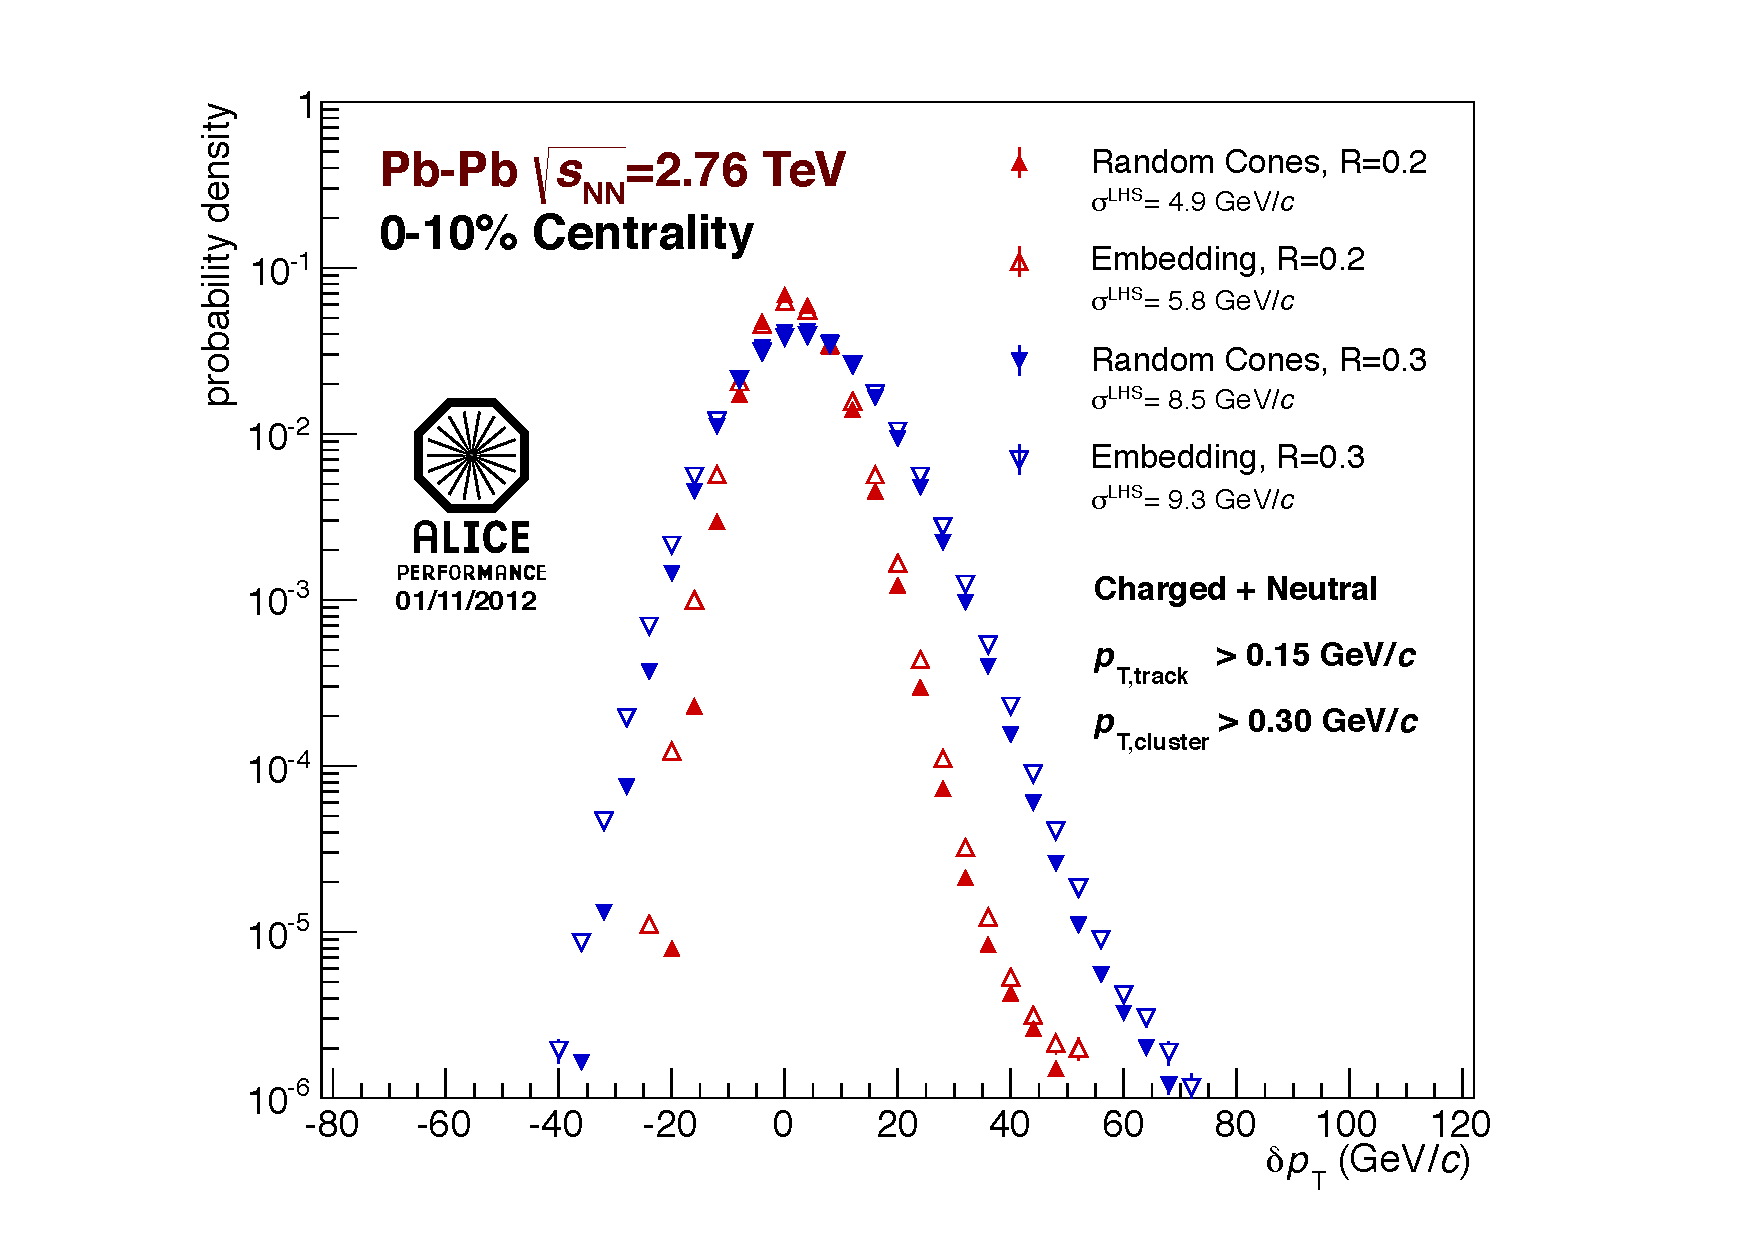
\includegraphics[width=0.5\textwidth]{DeltaPtFullV2}\hspace{2pc}
\begin{minipage}[b]{14pc}\caption{\dpT{} distributions for \mbox{Pb--Pb} collisions at $\snn=2.76$~TeV in the 0-10\% centrality class. 
Two different methods have been implemented: ``random cones'', shown with full symbols, and 
single particle embedding, shown with open symbols (see text for details);
 the distributions for $R=0.2$ are narrower w.r.t.~$R=0.3$ (color online).}
\label{fig:DeltaPtFullV2}
\end{minipage}
\end{figure}
\begin{comment}
Background fluctuations are the largest source of uncertainty in a heavy-ion jet
measurement. This is because the jet spectrum is a steeply falling function 
of the \pT{} and fluctuations in the background density may have
a big effect in its shape, especially for larger jet cone radii.
\end{comment}
Background fluctuations have been estimated in two different ways~\cite{bkg-alice-12}, namely using random cones
(scalar sum of the \pT{} of all particles found in a cone randomly placed in the event) and 
single particle embedding (with the \antikt{} algorithm).
\begin{comment}
one of which is independent of the particular jet finder choice (apart from the jet area scale), 
while the other makes use of the same algorithm employed to reconstruct signal jets. 

In the first method a random $\eta, \phi$ 
direction is thrown in the fiducial acceptance (the same used for signal jets)
and the \pT{} of all reconstructed particles in a cone of radius $R$ (``random cones'', RC) are summed up.
In the second method a high \pT{} particle or even a jet is randomly embedded in each event and
the clustering is done with the same algorithm use for signal jets.
\end{comment}
The residual \pT{} differences due to region-to-region fluctuations are calculated as:
$\delta p_{\rm T} = p_{\rm T,jet} - p_{\rm T,probe} -\rho \times A_{\rm jet}$, 
\begin{comment}
\begin{equation}
\delta p_{\rm T}^{\rm RC} = p_{\rm T}^{\rm RC} - \rho \times \pi R^2 \rm .
\label{eq:dptrc}
\end{equation}

The second method consists in running the same jet finder algorithm as
for signal jets after embedding in every event a high \pT{} particle or even a jet. 
In this case the \dpT{} distribution is calculated as:
\begin{equation}
\delta p_{\rm T} = p_{\rm T,jet} - p_{\rm T,probe} -\rho \times A_{\rm jet} \rm ,
\label{eq:dptemb}
\end{equation}
\end{comment}
where $p_{\rm T,probe}$ is the \pT{} of the embedded probe ($p_{\rm T,probe}=0$ for random cones).
The \dpT{} distributions, shown in Fig.~\ref{fig:DeltaPtFullV2}, tell us how much the jet \pT{} 
is smeared due to background fluctuations.

\begin{comment}
What we learn from \dpT{} distributions is how much the background \pT{} density fluctuates in each event. 
If the average background 
estimation is accurate, 
The \dpT{} distributions for the 0-10\% centrality events
are shown in Fig.~\ref{fig:DeltaPtFullV2}, where the two methods, random cones and single particle embedding,
are compared for two different radii, $R=0.2$, $0.3$. 
Both methods have advantages and disadvantages. The first method is much simpler 
and does not rely on any assumption about the structure of the background itself. The second method should be able reproduce
more carefully the background as seen by the \antikt{} algorithm; nevertheless embedding a high \pT{} particle may have
an effect on the clustering which is different from what one would expect from an actual jet. Embedding an entire jet would not completely solve
this issue as the problem of unambiguously matching the reconstructed jet with the probe jet would arise.
The random cone method is the nominal choice used in this measurement,
while the single particle embedding method gives the systematic uncertainty (on the order of 5\%).
\end{comment}

%\subsection{Detector response}
The detector response to jet reconstruction has been studied with pp simulated events, using the PYTHIA6~\cite{pythia6} generator
and the GEANT3~\cite{geant3} transport code.
\begin{comment}
To account for the reduced tracking efficiency due to the higher multiplicity in Pb--Pb collisions, 5\% of the 
tracks have been removed at detector level.
Apart from this correction for the tracking efficiency, the detector response to jet reconstruction is assumed 
to be the same as in the PYTHIA simulated proton-proton collisions.
\end{comment}
Jets are reconstructed both at generator level and at detector level. The generator-level and detector-level jets
are matched following a geometrical criterion. 

\begin{comment}
Particle-level jet A is matched with detector-level jet B if:
\begin{itemize}
\item $d({\rm A, B}) = \sqrt{(\eta_{\rm A}-\eta_{\rm B})^2 + (\phi_{\rm A}-\phi_{\rm B})^2} < 0.25$;
\item A is the nearest particle-level jet to B and B is the nearest detector-level jet to A (in the sense of the distance defined above).
\end{itemize}
When a valid matching is found, an entry is added to a fine-binned 2-dimensional histogram, 
having $p_{\rm T,jet}^{\rm rec}$ 
(reconstructed jet \pT) in the $x$ axis and $p_{\rm T,jet}^{\rm gen}$ (generated jet \pT) in the $y$ axis.

The same simulation gives the detector jet reconstruction efficiency which is found to be on the order of 
90\% at intermediate \pT{}, mainly due to the track reconstruction efficiency of the leading hadron (for leading hadron biased spectra).
\end{comment}

\section{Results}
\begin{comment}
\subsection{Unfolding}
\begin{figure}[t]
%\centering
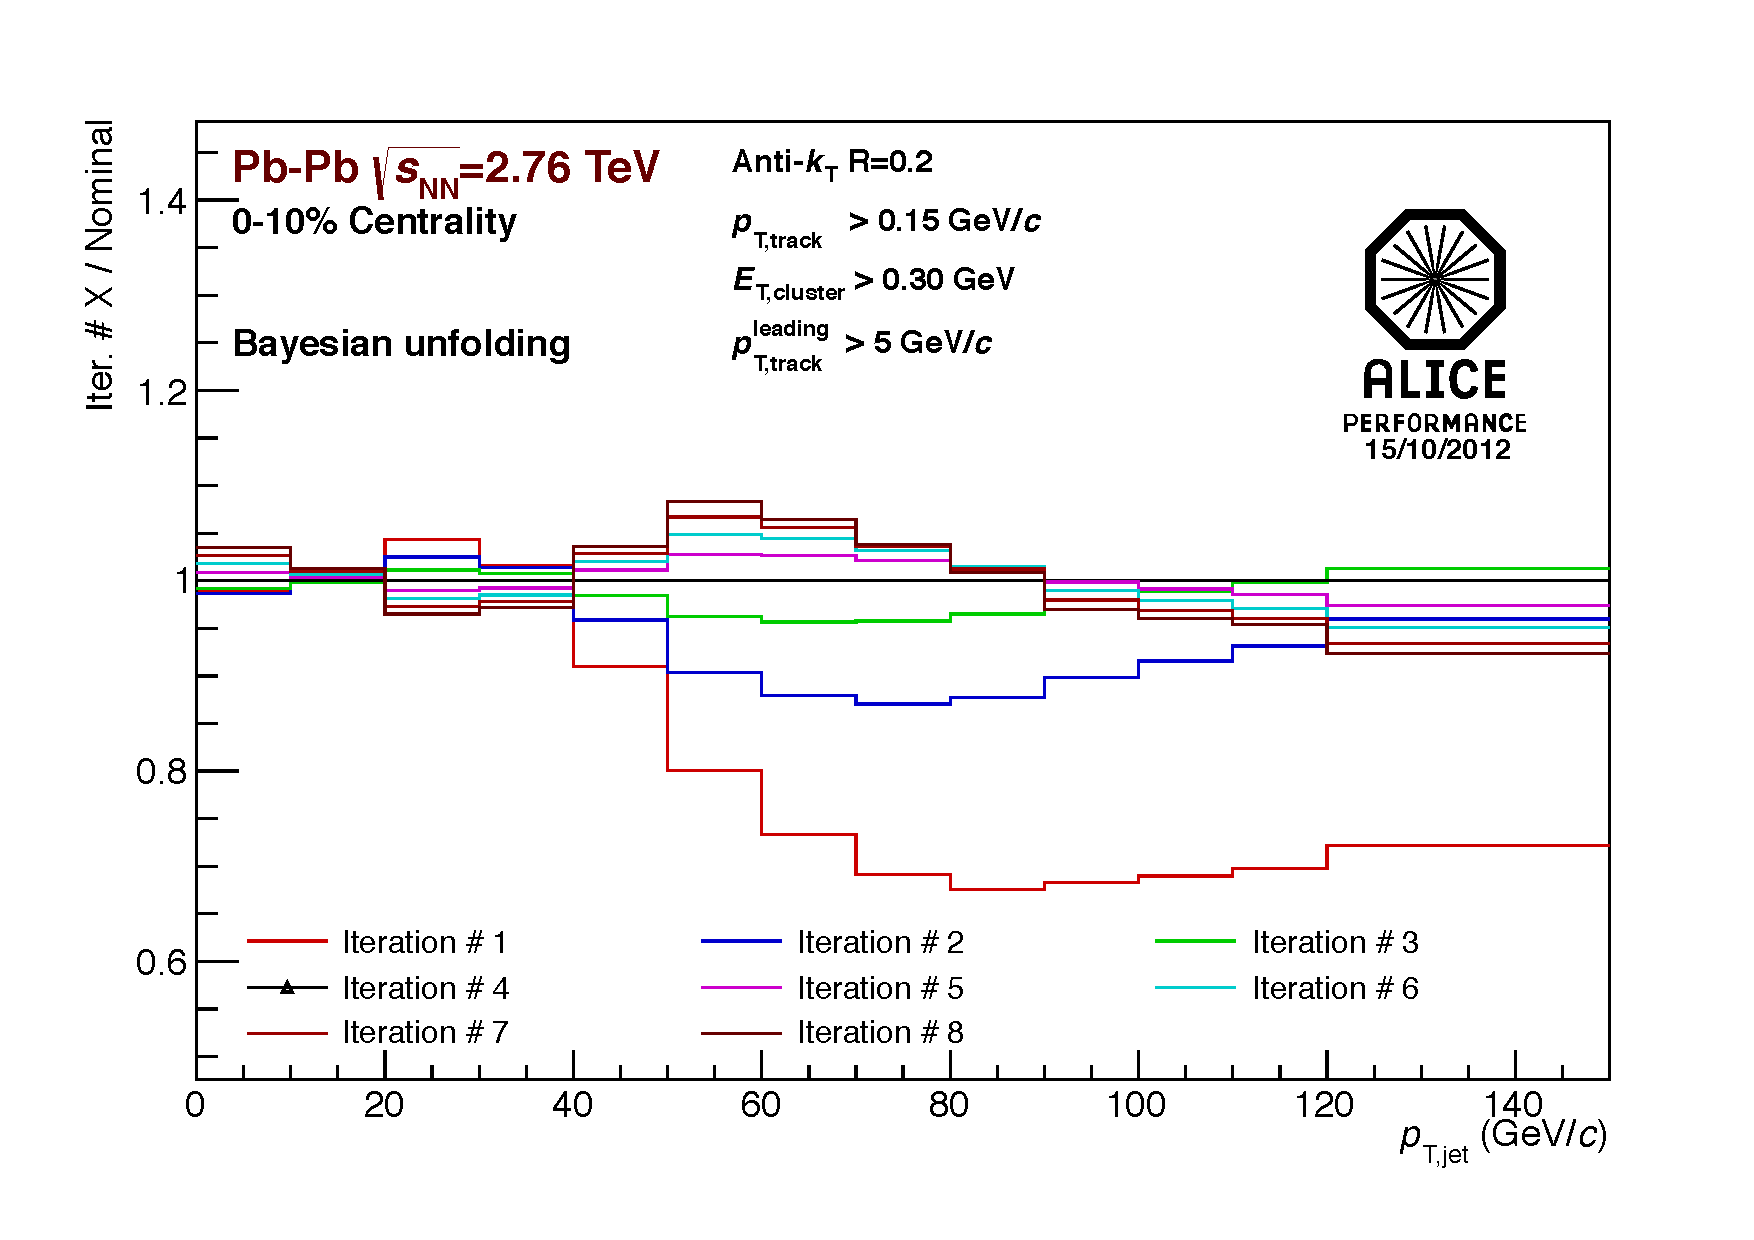
\includegraphics[width=0.56\textwidth]{IterComp_R02_Bias5}\hspace{2pc}
\begin{minipage}[b]{14pc}\caption{Bayesian unfolding of the \antikt{} ($R=0.2$) jet spectrum: from the 1st iteration to the 8th.}
\label{fig:IterComp_R02_Bias5}
\end{minipage}
\end{figure}
\end{comment}
This measurement makes use of the unfolding iterative method proposed by D'Agostini~\cite{bayes-dago-95}, which
contains elements of Bayesian statistics.
\begin{comment}
Here one starts with a set of initial probabilities 
$\boldsymbol \mu = (\m_1,\dots,\m_M)$ for an event to be found in each bin.
A smoothed version of the measured distribution is used as prior guess. 
These estimators are updated using the rule
\begin{equation}
\begin{split}
\hat{\mu}_i&=\frac{1}{\epsilon_i}\sum_{j=1}^{N}{P(\text{true value in bin}~i~|~\text{found in bin}~j)n_j} \\
&=\frac{1}{\epsilon_i}\sum_{j=1}^{N}\left( \frac{R_{ij}p_i}{\sum_k{R_{jk}p_k}} \right)n_j \rm .
\end{split}
\label{eq:eq001}
\end{equation}
Bayes' theorem formula is
\begin{equation}
P(C_i|E)=\frac{P(E|C_i)P(C_i)}{\sum_{l=1}^{n_C}{P(E|C_l)P(C_l)}} \rm ,
\end{equation}
where $P(C_i)$ and $P(E_j)$ are respectively the probability of the cause $i$ (true value in bin $i$) and
the probability of the event $j$ (value found in bin $j$). This formula has been used 
to derive eq.~\ref{eq:eq001}.
\end{comment}
In Bayesian unfolding the number of iterations plays the role of the regularization parameter. Based on 
the evolution of the covariance matrix and the converging of the solution itself, a number of four iterations
has been chosen as default. 
\begin{comment}
Figure~\ref{fig:IterComp_R02_Bias5} shows the ratio of the solutions obtained with a number of iterations
ranging from one to eight over the nominal solution. 
\end{comment}
Indeed after three/four iterations the procedure starts to converge. However, with more iterations
a characteristic fluctuation pattern does appear along with larger variances and (anti-)correlations between
far bins (indicating under-regularization).
Systematic uncertainties have been estimated taking into account variations
of the solution for $\pm 1$ iterations ($\sim 5\%$).

%\subsection{Leading hadron bias}

\begin{figure}[t]
\centering
%\subfloat[]
{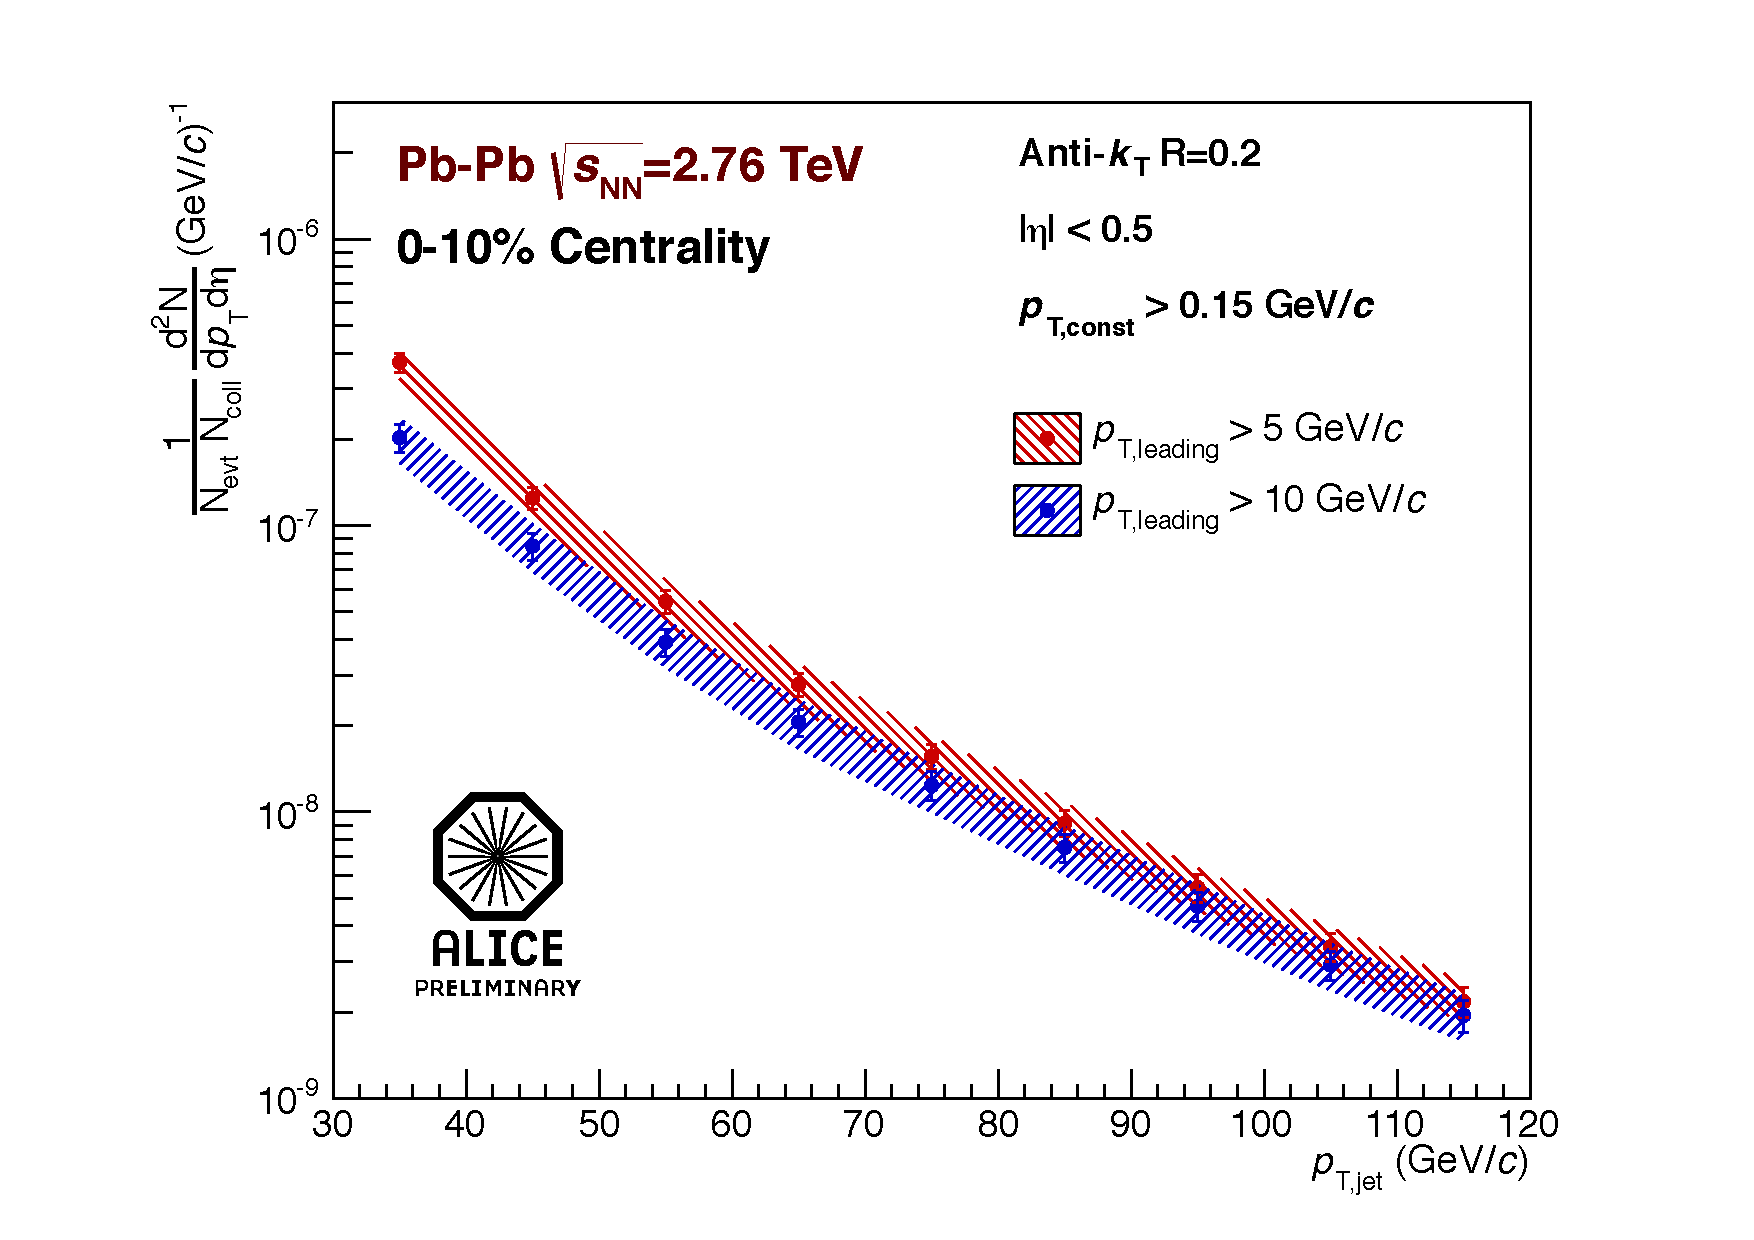
\includegraphics[width=.44\columnwidth]{FinalSpectraR02_5GeV_10GeV} } \quad %\label{fig:FinalSpectraLHR}} \quad
%\subfloat[]
{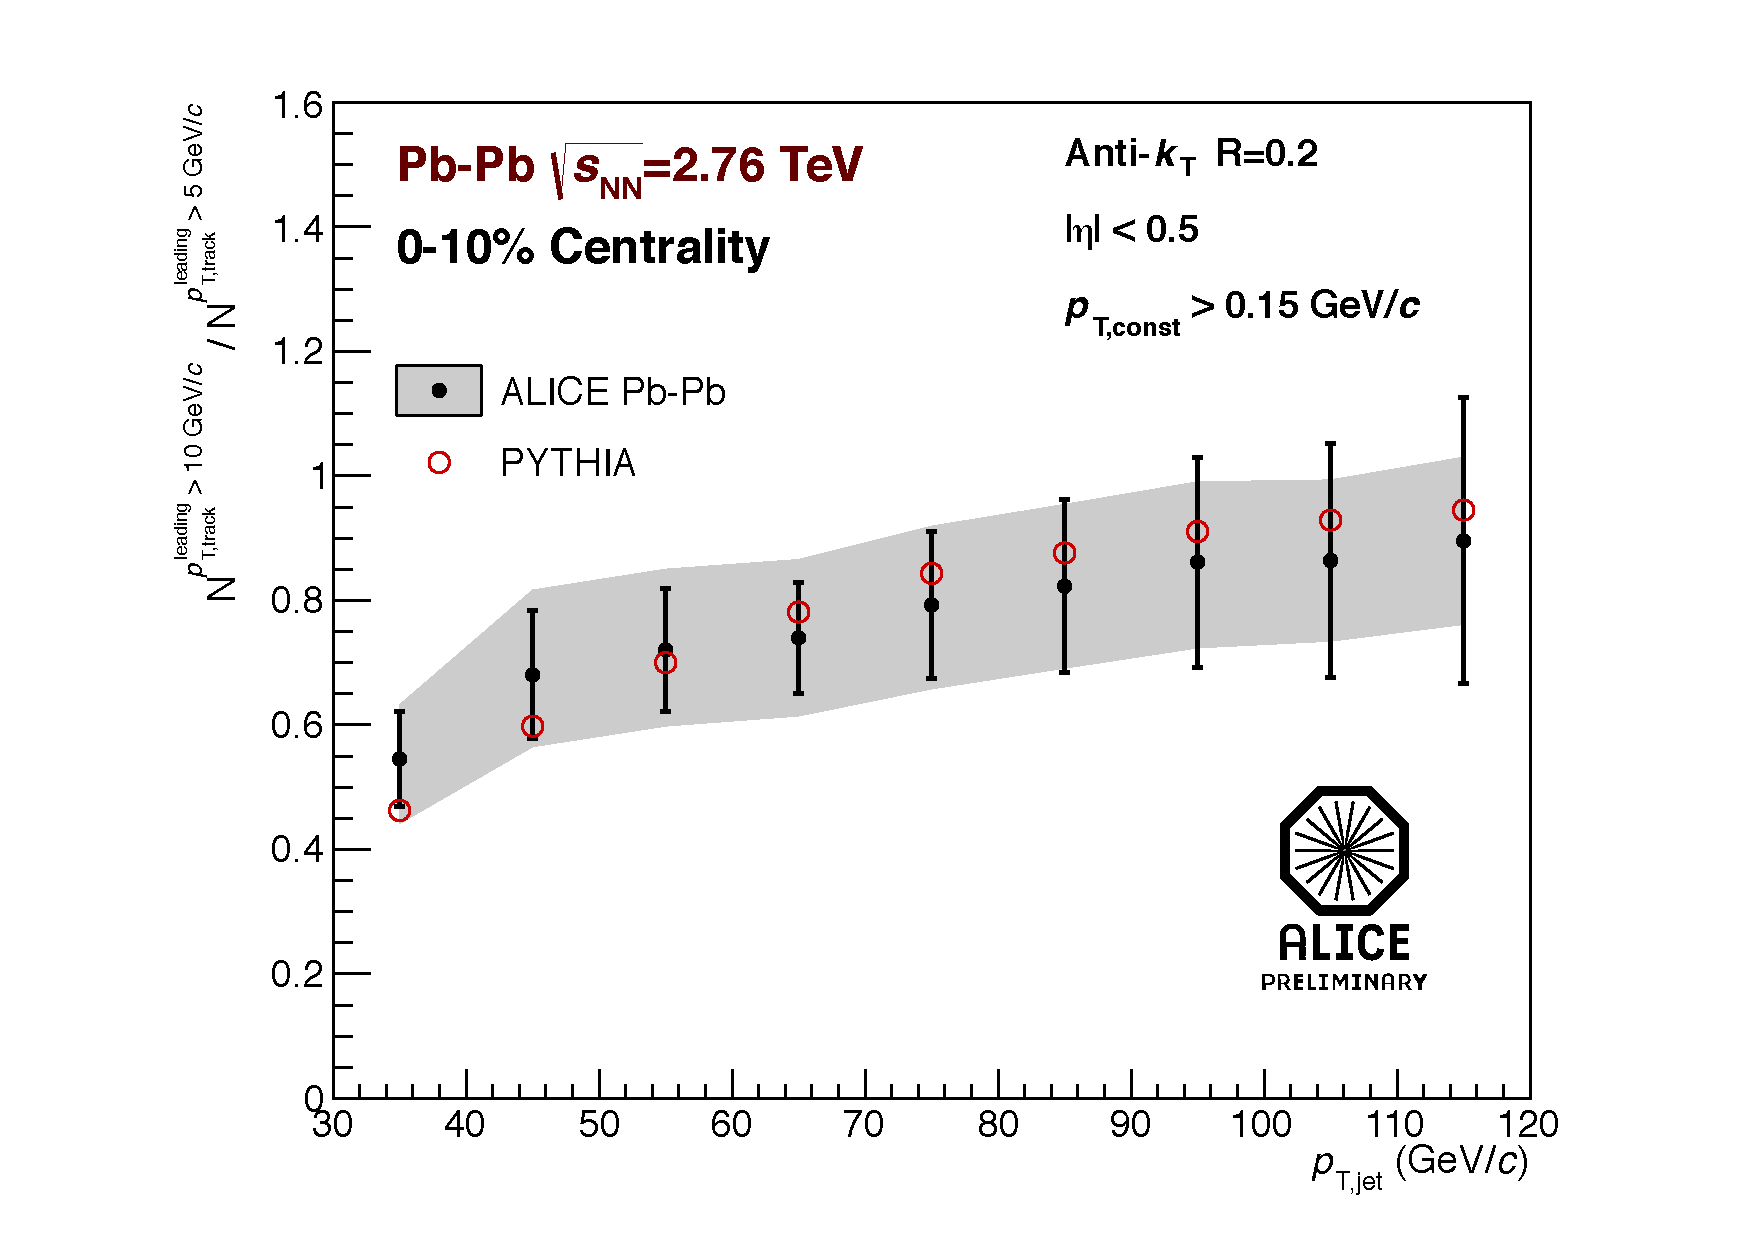
\includegraphics[width=.44\columnwidth]{FinalSpectraRatioR02_5GeV_10GeV} }%\label{fig:FinalSpectraLHRRatio}}
\caption{On the left: spectra of reconstructed jets in Pb--Pb collisions at $\snn=2.76$ TeV in the 0-10\% centrality class 
with two different minimum leading hadron \pT{} requirements.  On the right: ratio of the two spectra (solid circles) and comparison
 with a PYTHIA pp expectation (open circles). The bands represent the systematic uncertainty; statistical uncertainties
are shown with bars, when they are larger than markers (colors online).}
\label{fig:FinalSpectraLHRAndRatio}
\end{figure}

To better understand the effect of the leading hadron requirement
in the jet \pT{} spectrum, the analysis was performed for $p_{\rm T, leading} > 5,~10~\gevc$.
\begin{comment}
This is also a preliminary study that is especially useful for larger jet radii,
where a stronger bias may be needed in order to efficiently remove combinatorial jets.
\end{comment}
Figures~\ref{fig:FinalSpectraLHRAndRatio} show the two spectra with the two different leading hadron thresholds,
and the ratio, compared to a PYTHIA expectation. 
\begin{comment}
Statistical and systematic uncertainties on the ratio have
been computed taking into account that the two measurements come from the same data sample, and thus the 
uncertainties are partially correlated. 
The reasonable agreement with PYTHIA is consistent with a vacuum-like
fragmentation of the jet core.
\end{comment}

\section{Conclusions}
We have reported on the analysis techniques utilized to reconstruct jets in the 10\% most central Pb--Pb 
collisions at $\snn=2.76$~TeV recorded by ALICE in 2011. The raw jet \pT{} spectra are corrected for the average
background and biased requiring a minimum leading hadron \pT{}. Corrections
for background fluctuations and detector effects are applied via Bayesian unfolding.

The effect of the leading hadron requirement was studied for two different thresholds, 5~\gevc{} and 10~\gevc{}.
The ratio between the two corrected spectra is in reasonable agreement with a PYTHIA simulation, 
which indicates a vacuum-like fragmentation of the jet core.

\section*{References}
\bibliography{biblio}

\end{document}


